\documentclass[../dissertation.tex]{subfiles}
\begin{document}

\chapter{Review of the Field}

\section{Visualisation}

The visualisation of data is a field of critical importance that many huge companies rely on in order to make predictions, improve themselves, and get an edge over competitors. Data Visualisation is, "the presentation of data in a pictorial or graphical format [which] enables decision makers to see analytics presented visually, so they can grasp difficult concepts or identify new patterns.", as defined by SAS - a world leader in the field. This clearly defines Data Visualisation and how it is useful. 
\url{http://www.sas.com/en_us/insights/big-data/data-visualization.html}

Visualisation of data can be static or interactive, with interactive data able to give a user more information by, for example, selecting parts of the visualisation and getting more information on it, changing parameters for the visualisation and observing changes, or the moving of nodes in a network and seeing how the rest of the network responds. This can greatly improve the usefulness of the visualisation for users, with new trends or vulnerabilities becoming clearer faster through interacting with the visualisation. 

\section{Network Visualisation}

Network Visualisation is a branch of Data Visualisation involving the ability to display nodes and edges in a meaningful way to a user. This can be used for a large variety of purposes, such as to discover how information is grouped, how subsets of data interacts with other subsets, and how interconnected or isolated the data is.
\url{https://flowingdata.com/2010/11/17/why-network-visualization-is-useful/}

\section{Challenges of the Visualisation of Massive Networks in a Browser}

Visualisation of massive networks can lead to many challenges. Massive is a very vague term, but is generally considered as anything above about ten thousand <<source inserted here>>. These challenges generally present themselves in the form of computational challenges or visualisation challenges. Computational challenges are when the a system struggles to display a network visualisation due to lack of speed or performance from the CPU, RAM, backing storage or bandwidth. If a machine has a slow processor then the amount of time to create and then render the network will be increased greatly. Similarly, if the RAM installed is slow or if the network is big enough that it will not fit in the available amount of RAM, then the performance of the network visualisation will degrade greatly. 

The other computational challenge is the ability to store the network. Whether it is stored locally on a machine or stored somewhere on a network, this relies on fast disk access and enough storage space (which, depending on the amount of data that is to be stored to be visualised, could be nearly impossible to store on one machine). Hence, when storing several massive networks, they will always be held on the cloud, which means a high quality internet connection is required. 

Assuming that the machine is powerful enough in all of the above ways, and is capable of visualising massive networks, the next challenge is how to present that data in any meaningful way. When visualising a few hundred or thousand nodes, it is generally fairly easy to get useful information out of the visualisation. However, when a user is faced with a few hundred thousand nodes or even several million, it can be very difficult to gain any sort of insight from the visualisation. 

A goal of the project was to research techniques currently used to visualise massive networks, look into how successful they were, and then make a system that allows for the visualisation of massive networks in a browser and across a network. 

\section{Example within the Field}

\subsection{Visual Investigator}
Currently, Visual Investigator (a SAS product <<insert link for who SAS are>>) lets users view a network of entities in the system to see how they connect (for example: names, phone numbers and addresses). This works perfectly for a few entities, with useful information being shown clearly. However, with potentially millions of nodes, the network no longer shows any useful information - just a mass of nodes - and becomes unusably slow (Visual Investigator is a web app and both processing power and memory are hard limits which, depending on network size, will easily be hit).

As can be seen from the pictures below, the network starts out clear and load times are instant, but it soon becomes both meaningless and really slow. If there was a way to both speed up the loading times of huge networks, and make them convey meaningful information to the user, this would be very useful.

\begin{figure}
    \centering
    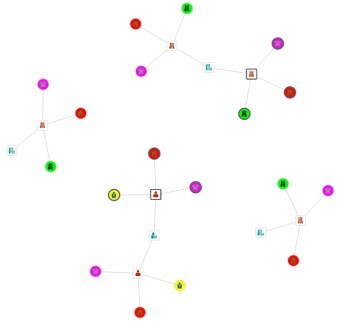
\includegraphics[width=9cm]{3/30_nodes}
    \caption{30 nodes, Load Time less than 1 second}
\end{figure}

\begin{figure}
    \centering
    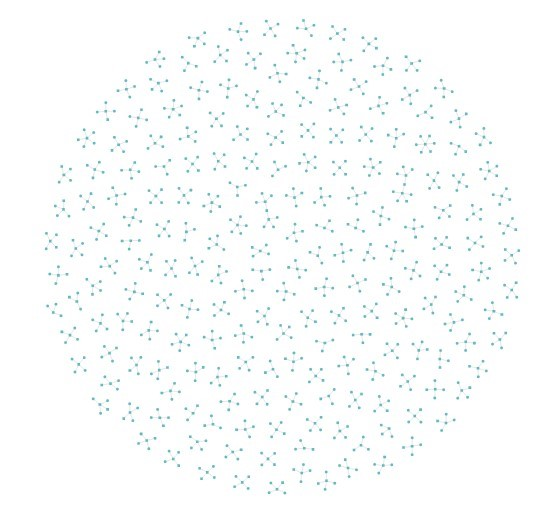
\includegraphics[width=9cm]{3/1000_nodes}
    \caption{1000 nodes, Load Time 10 seconds}
\end{figure}

\begin{figure}
    \centering
    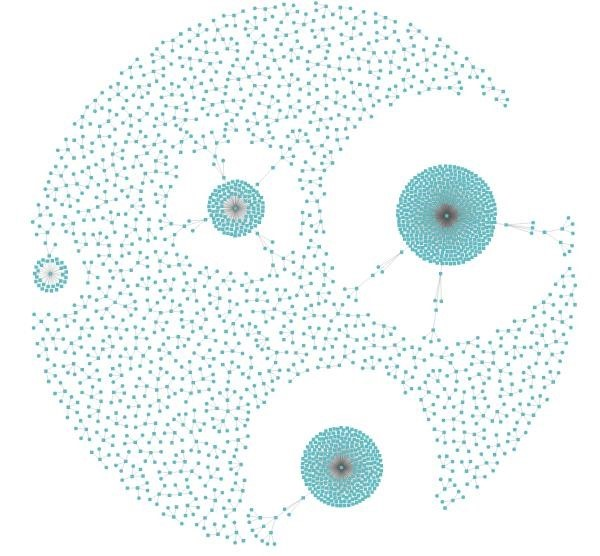
\includegraphics[width=9cm]{3/2500_nodes}
    \caption{2500 nodes, Load Time 30 seconds}
\end{figure}

\begin{figure}
    \centering
    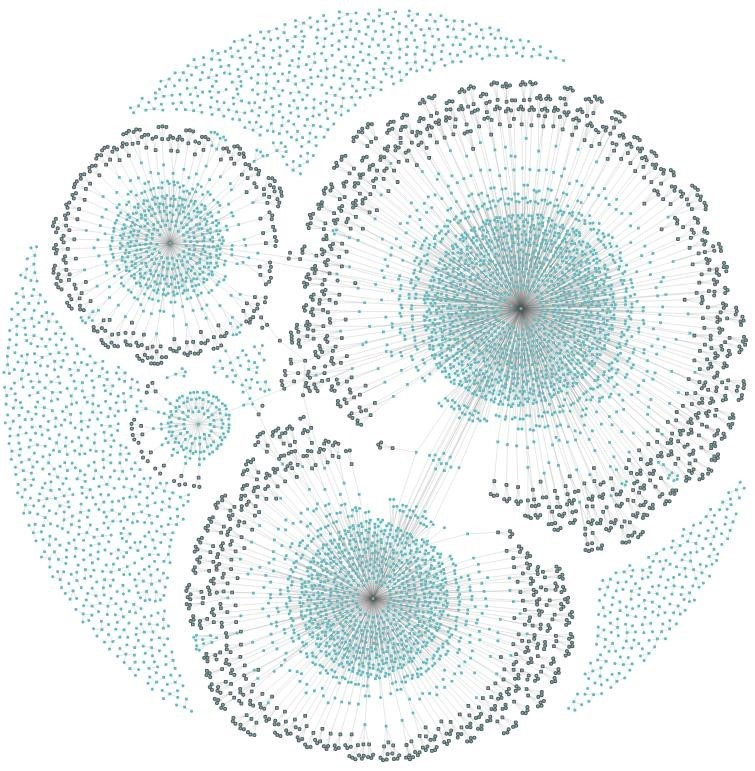
\includegraphics[width=9cm]{3/7500_nodes}
    \caption{7500 nodes, Load Time 300 seconds}
\end{figure}

\end{document}